\documentclass[11pt,a4paper]{article}

\usepackage[T1]{fontenc}
\usepackage[utf8]{inputenc}
\usepackage{lmodern}
\usepackage[margin=2.4cm]{geometry}
\usepackage{microtype}
\usepackage{amsmath,amssymb}
\usepackage{booktabs}
\usepackage{siunitx}
\usepackage{graphicx}
\usepackage{subcaption}
\usepackage{listings}
\usepackage{float}
\usepackage{placeins}
\usepackage{xcolor}
\usepackage{enumitem}
\usepackage{tikz}
\usetikzlibrary{arrows.meta,positioning}
\usepackage[hidelinks]{hyperref}
\usepackage{caption}
\captionsetup{font=small,labelfont=bf}
\renewcommand{\arraystretch}{1.22}

\sisetup{detect-weight=true,detect-family=true,group-separator={,},group-minimum-digits=4}
\setlist[itemize]{leftmargin=1.4em,itemsep=2pt,topsep=2pt}
\setlist[enumerate]{leftmargin=1.6em,itemsep=2pt,topsep=2pt}

\newcommand{\code}[1]{\texttt{#1}}

\lstset{
  basicstyle=\ttfamily\footnotesize,
  keywordstyle=\color{blue!70!black},
  commentstyle=\color{green!40!black},
  frame=single,
  framerule=0.3pt,
  columns=fullflexible,
  keepspaces=true,
  showstringspaces=false,
  breaklines=true
}

\title{\textbf{Andas: A Columnar, Streaming Data Processing Library for Android}\\[0.4em]
\large Technical Report on CSV Ingestion, Computation, and Performance Evaluation}
\author{Andas Engineering Team}
\date{November 1, 2026}

\hypersetup{
  pdftitle={Andas: A Columnar, Streaming Data Processing Library for Android},
  pdfauthor={Andas Engineering Team},
  pdfsubject={Technical report: CSV ingestion, columnar computation, performance evaluation},
  pdfkeywords={Android, data processing, CSV, columnar storage, JVM, performance}
}

\begin{document}
\maketitle

\begin{abstract}
Andas is an Android library that brings a pandas-like data-analysis API to Kotlin and Java.
The previous implementation materialized an entire CSV file as a list of strings, constructed
a map per row, and then transposed the rows into columns; each column also kept a private copy
of the index and a label-to-position hash map.  On a 192\,MB Android heap this design ran out of
memory at 100k rows $\times$ 15 columns.  We redesigned the ingestion and computation paths around
streaming parsing, columnar primitive storage, a shared range index, and algorithmically improved
operators.  We evaluate the optimized library on a JVM and on an Android ARM64 emulator, and compare
it with pandas 2.1.0 on the same machine and datasets.  On the JVM, the optimized reader completes
200k rows $\times$ 15 columns (36\,MB) in 1.44\,s with 56\,MB of retained heap, whereas the baseline
fails with an out-of-memory error at the same size.  On the Android emulator, the baseline fails at
100k rows and the optimized reader completes 200k rows with 35\,MB of retained heap.  At 50k rows,
statistical, sorting, and join operations improve by 7--33$\times$ over the baseline; filtering and
grouped aggregation improve by 2.9$\times$ and 1.4$\times$, respectively.  Compared with pandas, the
optimized reader is still 3.2--6.0$\times$ slower on the desktop JVM but uses less memory, while
computation kernels remain 6--20$\times$ slower, pointing to native columnar kernels as future work.  A 35-metric cross-language consistency
check (pandas vs JVM vs Android) passes on both runtimes with a maximum relative error of
$3.17\times10^{-15}$.
\end{abstract}

\noindent\textbf{Keywords:} Android, CSV parsing, columnar storage, JVM performance, pandas, data analysis.

\section{Introduction}

Data analysis on Android is usually performed either on a remote service or with ad-hoc
collections and loops.  Andas explores a third option: a local, pandas-like library for Kotlin
and Java, implemented as a small JVM API with optional JNI acceleration.  The library supports
\code{Series}, \code{DataFrame}, selection, filtering, sorting, grouping, joins, null handling,
asynchronous I/O, and CSV import/export.

The first release prioritized API coverage.  Its CSV reader followed a conventional but
memory-hungry pipeline: the file was read into a \code{List<String>}, each line was parsed into
a \code{Map<String, Any?>}, and the list of maps was transposed into column-oriented
\code{Series} objects.  This pipeline is acceptable for small examples but not for the workloads
that motivate a data library.  In our measurements, a 36\,MB file with 200k rows and 15 columns
could not be read on a 192\,MB Android heap, and even on a 256\,MB JVM heap it failed at 200k rows.
The same design also resulted in slow statistical kernels, quadratic sorting, and quadratic joins.

This report describes the redesign, measures it, and compares it with pandas as a reference
implementation.  The contributions are:
\begin{itemize}
  \item a streaming, column-oriented CSV parser that never materializes the whole file or row maps;
  \item primitive column storage (\code{IntArray}, \code{LongArray}, \code{DoubleArray},
        \code{BooleanArray}) with a nullable bitmap, plus a shared $O(1)$-memory range index;
  \item algorithmic rewrites of statistics, sorting, filtering, grouping, and joins;
  \item an evaluation on the JVM and Android, including memory, out-of-memory thresholds,
        and a pandas comparison.
\end{itemize}

The implementation is available at \url{https://github.com/trueWangSyutung/Andas} and is released
as version 0.2.1.  The raw results, scripts, and figures are included in the repository under
\code{bench/}.

\section{Background and Motivation}

\subsection{Android memory constraints}

Android applications run on ART with a per-application heap limit.  The limit depends on the device
and on whether \code{android:largeHeap} is requested; in our API-36 ARM64 emulator,
\code{Runtime.maxMemory()} reports 192\,MB.  A data library must therefore keep the live set small
and avoid transient object graphs that are several times larger than the input.  The legacy
pipeline violated both requirements: it created one map entry per cell during parsing, retained the
entire row representation, and then created a second column representation.

\subsection{Legacy pipeline}

For $n$ rows and $m$ columns, the legacy reader performed the following steps:
\begin{enumerate}
  \item read the whole file into \code{List<String>} (one string per line);
  \item for each line, split fields into a \code{List<String>}, then build a
        \code{Map<String, Any?>} with $m$ entries;
  \item for each column, scan all row maps and build a \code{Series}, copying the data list;
  \item create a default index list of $n$ boxed integers for every column and a
        \code{HashMap} from label to position for every column.
\end{enumerate}
The row maps, boxed numeric values, duplicated indices, and transposition copy dominate both
time and memory.  In addition, type inference used only the first data row, so a leading empty
value could turn a numeric column into a string column.

\section{Design and Implementation}

\subsection{Streaming, columnar CSV ingestion}

The new reader is implemented in \code{CsvReader}.  It reads characters through a 64\,KB buffer
and feeds a small state machine that understands quoted fields, escaped quotes (\code{""}),
embedded commas and newlines, CRLF, a UTF-8 BOM, and blank lines.  Fields are appended to reusable
buffers; the parser does not allocate a string for every numeric cell.

Column types are inferred from up to 64 sample records.  The inference merges the observed kinds
(int, long, double, boolean, date, string) and selects the narrowest common type.  If a later value
cannot be parsed according to the inferred type, the column is promoted to string storage so that
no data are lost.  Duplicate headers are disambiguated (\code{a}, \code{a} becomes \code{a},
\code{a\_1}).

Figure~\ref{fig:pipeline} shows the ingestion pipeline.  A column builder appends directly into
primitive arrays; a null bitmap is allocated only when the first null is observed.  At the end,
the builders produce \code{Series} objects that share a single index instance.

\begin{figure}[H]
\centering
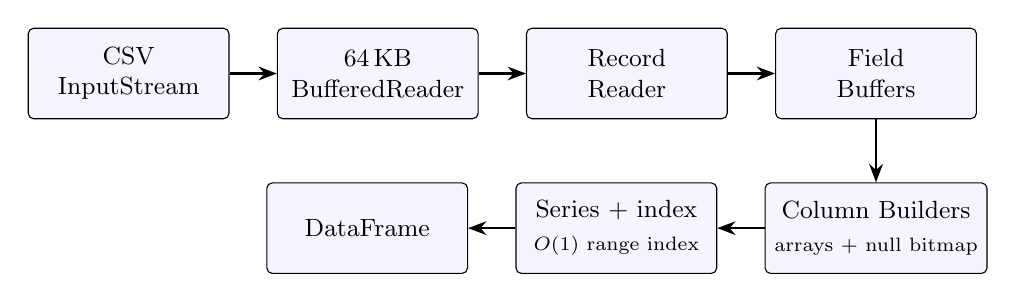
\begin{tikzpicture}[
  font=\small, >=Stealth,
  box/.style={draw, rounded corners=2pt, align=center, minimum width=2.55cm,
              minimum height=1.15cm, fill=blue!4},
  arr/.style={->, thick}
]
  \node[box] (in) {CSV\\InputStream};
  \node[box, right=6mm of in] (br) {64\,KB\\BufferedReader};
  \node[box, right=6mm of br] (rr) {Record\\Reader};
  \node[box, right=6mm of rr] (fb) {Field\\Buffers};
  \node[box, below=8mm of fb] (cb) {Column Builders\\[1pt]{\scriptsize arrays + null bitmap}};
  \node[box, left=6mm of cb] (se) {Series + index\\[1pt]{\scriptsize $O(1)$ range index}};
  \node[box, left=6mm of se] (df) {DataFrame};
  \draw[arr] (in) -- (br);
  \draw[arr] (br) -- (rr);
  \draw[arr] (rr) -- (fb);
  \draw[arr] (fb) -- (cb);
  \draw[arr] (cb) -- (se);
  \draw[arr] (se) -- (df);
\end{tikzpicture}
\caption{Streaming, columnar CSV ingestion.  No row maps or full-file string list are created.}
\label{fig:pipeline}
\end{figure}

The core loop is intentionally simple; all complexity is hidden in the record reader and the
column builders.

\begin{lstlisting}[language=C++]
while (reader.nextRecord()) {
  for (int c = 0; c < columnCount; ++c) {
    if (c < reader.fieldCount())
      builders[c].append(reader.field(c));
    else
      builders[c].appendNull();
  }
}
return DataFrame::fromColumnar(builders, RangeIndex::of(rowCount));
\end{lstlisting}

Batched ingestion uses the same parser with a row-count trigger: every batch is converted into an
independent \code{DataFrame} and handed to a callback, so peak memory is bounded by the batch size
rather than by the file size.

\subsection{Shared index and lazy label mapping}

Every column of a \code{DataFrame} shares the same index object.  For the common default index
$0,\ldots,n-1$, \code{RangeIndexList} stores only the size and computes labels on demand, taking
$O(1)$ memory instead of $O(n)$ boxed integers.  Custom string or integer labels are stored once
and shared by all columns.  The label-to-position \code{HashMap} is built lazily, only when a
label lookup is actually requested; positional access, which dominates computation, never needs it.

\subsection{Primitive column storage}

Numeric and boolean columns are stored in primitive arrays.  When a column contains nulls, a
\code{BooleanArray} bitmap marks present positions; otherwise the bitmap is omitted.  The public
\code{List<T?>} view is a lightweight adapter that boxes values only when a caller explicitly reads
them through the \code{List} interface.  Internal kernels use the arrays directly, avoiding both
boxing and intermediate lists.

\subsection{Algorithmic rewrites}

Table~\ref{tab:design} summarizes the changes.  The common theme is to remove intermediate
collections and to replace quadratic scans with sorting or hashing.

\begin{table}[H]
\centering
\small
\caption{Legacy versus optimized implementation.}
\label{tab:design}
\begin{tabular}{@{}p{0.27\linewidth}p{0.31\linewidth}p{0.34\linewidth}@{}}
\toprule
Operation & Legacy & Optimized \\
\midrule
Read & whole file as strings, row maps, transpose & streaming records into primitive columns \\
Index & per-column list and hash map & shared range index, lazy map \\
Statistics & \code{filterNotNull $\to$ map $\to$ toDoubleArray} & single pass over primitive arrays \\
Sort & string comparison, \code{indexOf} per row ($O(n^2)$) & numeric sort ($O(n\log n)$), stable row permutation \\
Filter & full row maps and per-cell \code{Series} & lazy row view, position mask \\
Group-by & per-group temporary \code{DataFrame} & one hash grouping and one aggregation scan \\
Join & nested loops ($O(nm)$) & hash join ($O(n+m)$) \\
Export & unbuffered, unescaped writes & buffered writer with CSV escaping \\
\bottomrule
\end{tabular}
\end{table}

The statistical kernels traverse a column once.  Variance and standard deviation use Welford's
online algorithm, which avoids the cancellation error of the naive sum-of-squares formula and
allows the mean and variance to be computed in the same pass.  Sorting compares numeric values
numerically (the legacy Kotlin fallback compared their string representations), places nulls last,
and builds the output columns by permutation rather than by repeated label lookups.  Filtering
collects positions and projects the columns once.  Grouped aggregation hashes the group key once
and aggregates all requested columns in a second pass.  Joins build a hash table on one side and
probe it with the other.

\subsection{Native layer and OpenMP}

The optional JNI layer exposes array kernels for sums, means, extrema, normalization, dot products,
norms, sorting indices, null handling, and grouping.  We enabled OpenMP in the CMake build via
\code{find\_package(OpenMP)}; if OpenMP is unavailable, the build falls back to serial code.  We also
fixed index-order bugs in the parallel implementations of \code{findNullIndices},
\code{dropNullValues}, \code{where}, and \code{mergeIndices}: merging per-thread vectors under a
critical section does not preserve index order, which silently misaligned rows.

\subsection{Compatibility and correctness}

The public API is preserved: existing constructors, \code{readCSV}, \code{sum}, \code{sortValues},
\code{groupBy}, \code{merge}, and asynchronous helpers keep their signatures.  The implementation
adds regression tests for quoted fields, embedded newlines, duplicate headers, missing columns,
type promotion, null handling, numeric sorting, grouped aggregation, joins, correlation, and
normalization.  On the JVM, 32 tests pass and 9 JNI-only tests are skipped because the native
library is not available; the Android instrumentation test exercises the reader on the emulator.

\section{Experimental Methodology}

\subsection{Environment}

Experiments run on an Apple M2 machine with macOS 27.0.1, OpenJDK 21.0.12, Gradle 8.13, AGP 8.13.2,
and Kotlin 2.0.21.  Android measurements use an API-36 ARM64 emulator (AVD \code{MullionFold76})
whose reported maximum heap is 192\,MB.  The pandas reference runs on CPython 3.10.11 with pandas
2.1.0 and the NumPy C engine.

\subsection{Datasets}

We generated deterministic synthetic CSV files whose schema mirrors the project's 37\,MB
\code{largest.csv}: three 10-character string columns (the third has 10 categories), three 12-digit
integer columns, three small integer columns, three double columns, and three float columns.
Row counts are 10k, 25k, 50k, 100k, and 200k; the largest file is approximately 36\,MB.  A separate
join benchmark uses two 5k-row tables with an integer key.  The generation script fixes the random
seed, so all implementations read identical bytes.  All files are on local disk and the page cache
is warm before each measured run.

\subsection{Baseline and variants}

The baseline is commit \code{9bb6715}, the last revision before this work, checked out in a separate
Git worktree.  On the JVM the native library is unavailable; we wrap the baseline's
\code{System.loadLibrary} calls in a try/catch so that the baseline falls back to its Kotlin paths
instead of aborting during class initialization.  This patch is used only for JVM experiments.
On Android the baseline is built unmodified and uses its JNI layer.

\subsection{Metrics and protocol}

\begin{itemize}
  \item \textbf{Read time}: wall-clock time of \code{DataFrameIO.readCSV(File)}.  Each size runs in
        three independent JVMs (or Python processes) and we report the median.  A 10k-row file
        warms the parser and the JIT before the measured read.
  \item \textbf{Retained heap}: \code{totalMemory - freeMemory} after \code{System.gc()} and a
        120\,ms pause.  For pandas we report the incremental resident set size (RSS) after the read;
        the two metrics are related but not identical.
  \item \textbf{Peak heap}: a sampler thread polls \code{MemoryMXBean} every 50\,ms during the
        measured read and records the maximum.  This is an upper bound on heap usage during the
        read, not a retained-set measurement.
  \item \textbf{Operation time}: after reading 50k rows, a warm-up operation is executed, then a
        second operation is timed; three independent JVMs provide the median.
  \item \textbf{Out of memory}: a run is marked OOM when an \code{OutOfMemoryError} is thrown.
        JVM reads use \code{-Xmx256m}; Android uses the emulator's 192\,MB heap.
\end{itemize}

\section{Results}

\subsection{JVM CSV read scalability}

Table~\ref{tab:jvmread} and Figure~\ref{fig:jvmread} report read time, retained heap, and sampled
peak heap.  The baseline grows faster than linearly in time and memory; the optimized reader remains
roughly linear and still completes at 200k rows.

\begin{table}[H]
\centering
\small
\caption{JVM CSV read performance (36\,MB at 200k rows, 15 columns, \code{-Xmx256m}).}
\label{tab:jvmread}
\begin{tabular}{@{}rrrrrrrr@{}}
\toprule
Rows & \multicolumn{2}{c}{Time (ms)} & & \multicolumn{2}{c}{Retained (MB)} & \multicolumn{2}{c}{Peak (MB)} \\
\cmidrule(lr){2-3}\cmidrule(lr){5-6}\cmidrule(lr){7-8}
 & Base & Opt. & Speedup & Base & Opt. & Base & Opt. \\
\midrule
10k  & 321  & 138  & 2.33$\times$ & 15  & 4  & 88  & 41 \\
25k  & 623  & 244  & 2.55$\times$ & 36  & 8  & 137 & 119 \\
50k  & 1071 & 541  & 1.98$\times$ & 78  & 14 & 165 & 141 \\
100k & 2540 & 964  & 2.63$\times$ & 155 & 30 & 245 & 162 \\
200k & OOM  & 1440 & --           & OOM & 56 & OOM & 214 \\
\bottomrule
\end{tabular}
\end{table}

\begin{figure}[H]
\centering
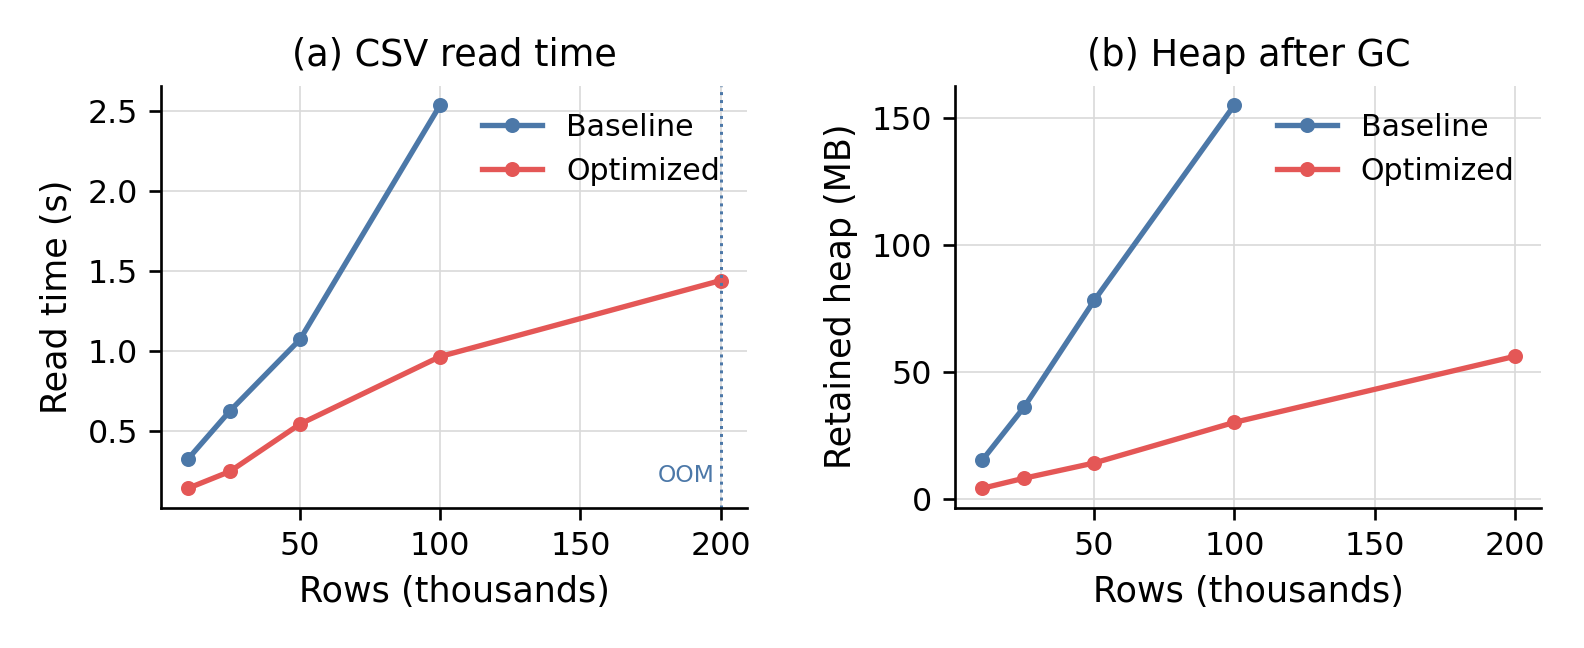
\includegraphics[width=0.95\linewidth]{figures/fig_report_jvm.png}
\caption{JVM CSV read scaling: (a) read time; (b) retained heap after GC.  The baseline fails at
200k rows under a 256\,MB heap.}
\label{fig:jvmread}
\end{figure}

The optimized reader uses 3--5$\times$ less retained heap at the same row count.  At 100k rows the
retained heap falls from 155\,MB to 30\,MB, and the baseline's 200k run cannot complete.  The
optimized peak at 200k (214\,MB) is close to the heap limit, but the retained set after GC is only
56\,MB; the difference is allocation churn from string cells and array growth, not live data.
\subsection{Computation kernels}

Table~\ref{tab:ops} and Figure~\ref{fig:ops} report operation time at 50k rows.  Statistical
kernels improve by 7--30$\times$, sorting by 32.9$\times$, and the 5k $\times$ 5k join by
30.9$\times$.  Filtering improves by 2.9$\times$ because the legacy implementation still performs a
linear scan and the optimized path adds column projection.  Grouped sum improves by only 1.4$\times$
because the legacy fallback was already a hash aggregation; this is expected and shows that the
gains come from data structures and algorithms rather than from uniformly replacing code with JNI.

\begin{table}[H]
\centering
\small
\caption{Operation time at 50k rows (merge: 5k $\times$ 5k).}
\label{tab:ops}
\begin{tabular}{@{}lrrr@{}}
\toprule
Operation & Baseline (ms) & Optimized (ms) & Speedup \\
\midrule
\code{sum}             & 30   & 1  & 30.0$\times$ \\
\code{mean}            & 28   & 2  & 14.0$\times$ \\
\code{std}             & 28   & 4  & 7.0$\times$ \\
\code{describe}        & 80   & 3  & 26.7$\times$ \\
\code{sortValues}      & 2629 & 80 & 32.9$\times$ \\
\code{filterGreaterThan} & 23 & 8  & 2.9$\times$ \\
\code{groupBySum}      & 27   & 20 & 1.4$\times$ \\
\code{merge}           & 557  & 18 & 30.9$\times$ \\
\bottomrule
\end{tabular}
\end{table}

\begin{figure}[H]
\centering
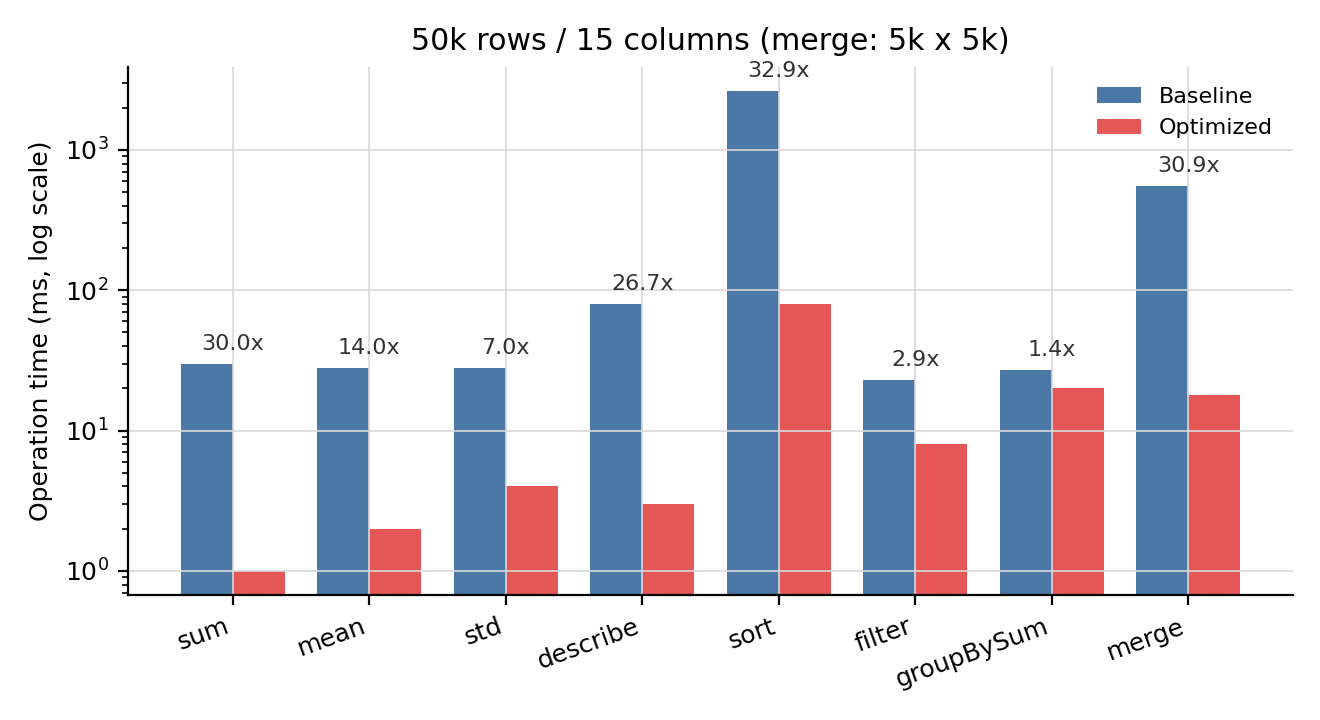
\includegraphics[width=0.85\linewidth]{figures/fig_ops_time.png}
\caption{Operation time for the baseline and the optimized implementation (log scale).}
\label{fig:ops}
\end{figure}

A correctness check confirms the sorting change: the legacy Kotlin fallback sorts
\code{double\_col\_10} lexicographically and returns $-0.0166$ as the first value on the 50k
dataset, while the optimized implementation returns $-99.9979$ and produces a monotonically
non-decreasing numeric sequence.  The legacy native sort also drops nulls before computing the
permutation, which misaligns rows when the sort column contains nulls.

\subsection{Comparison with pandas}

pandas is the direct design reference for Andas.  We ran pandas 2.1.0 on the same machine and the
same CSV files, using \code{pd.read\_csv(..., engine="c")}.  Each measurement uses a fresh Python
process; a 10k read warms the C parser, then the target file is read.  Table~\ref{tab:pandasread}
and Figure~\ref{fig:pandasread} report read time; Table~\ref{tab:pandasops} and Figure~\ref{fig:pandasops} report operations.

\begin{table}[H]
\centering
\small
\caption{Read comparison with pandas 2.1.0 (same machine and files).}
\label{tab:pandasread}
\begin{tabular}{@{}rrrrrr@{}}
\toprule
Rows & Baseline (ms) & Optimized (ms) & pandas (ms) & Opt./pandas & Base/pandas \\
\midrule
10k  & 321  & 138  & 22.9  & 6.02$\times$ slower & 14.0$\times$ slower \\
25k  & 623  & 244  & 56.4  & 4.32$\times$ slower & 11.0$\times$ slower \\
50k  & 1071 & 541  & 112.8 & 4.80$\times$ slower & 9.50$\times$ slower \\
100k & 2540 & 964  & 239.6 & 4.02$\times$ slower & 10.6$\times$ slower \\
200k & OOM  & 1440 & 446.7 & 3.22$\times$ slower & OOM \\
\bottomrule
\end{tabular}
\end{table}

\begin{table}[H]
\centering
\small
\caption{Operation comparison with pandas 2.1.0 at 50k rows (merge: 5k $\times$ 5k).}
\label{tab:pandasops}
\begin{tabular}{@{}lrrrr@{}}
\toprule
Operation & Baseline (ms) & Optimized (ms) & pandas (ms) & Opt./pandas \\
\midrule
\code{sum}        & 30   & 1  & 0.12  & 8.3$\times$ slower \\
\code{mean}       & 28   & 2  & 0.10  & 20.0$\times$ slower \\
\code{std}        & 28   & 4  & 0.37  & 10.8$\times$ slower \\
\code{describe}   & 80   & 3  & 3.22  & 0.93$\times$ (slightly faster) \\
\code{sortValues} & 2629 & 80 & 12.67 & 6.3$\times$ slower \\
\code{filter}     & 23   & 8  & 0.55  & 14.5$\times$ slower \\
\code{groupBy}    & 27   & 20 & 1.85  & 10.8$\times$ slower \\
\code{merge}      & 557  & 18 & 1.43  & 12.6$\times$ slower \\
\bottomrule
\end{tabular}
\end{table}

\begin{figure}[H]
\centering
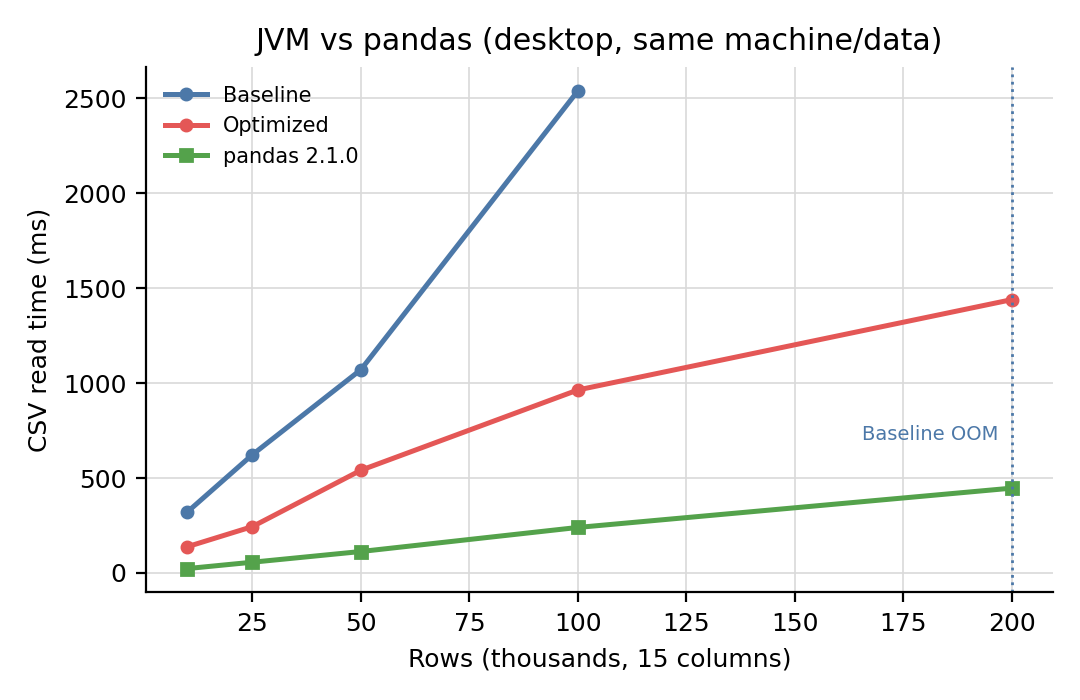
\includegraphics[width=0.82\linewidth]{figures/fig_read_time_pandas.png}
\caption{Read-time comparison with pandas 2.1.0.  pandas uses a C parser and NumPy arrays; the
runtimes differ, so the comparison indicates order of magnitude only.}
\label{fig:pandasread}
\end{figure}

\begin{figure}[H]
\centering
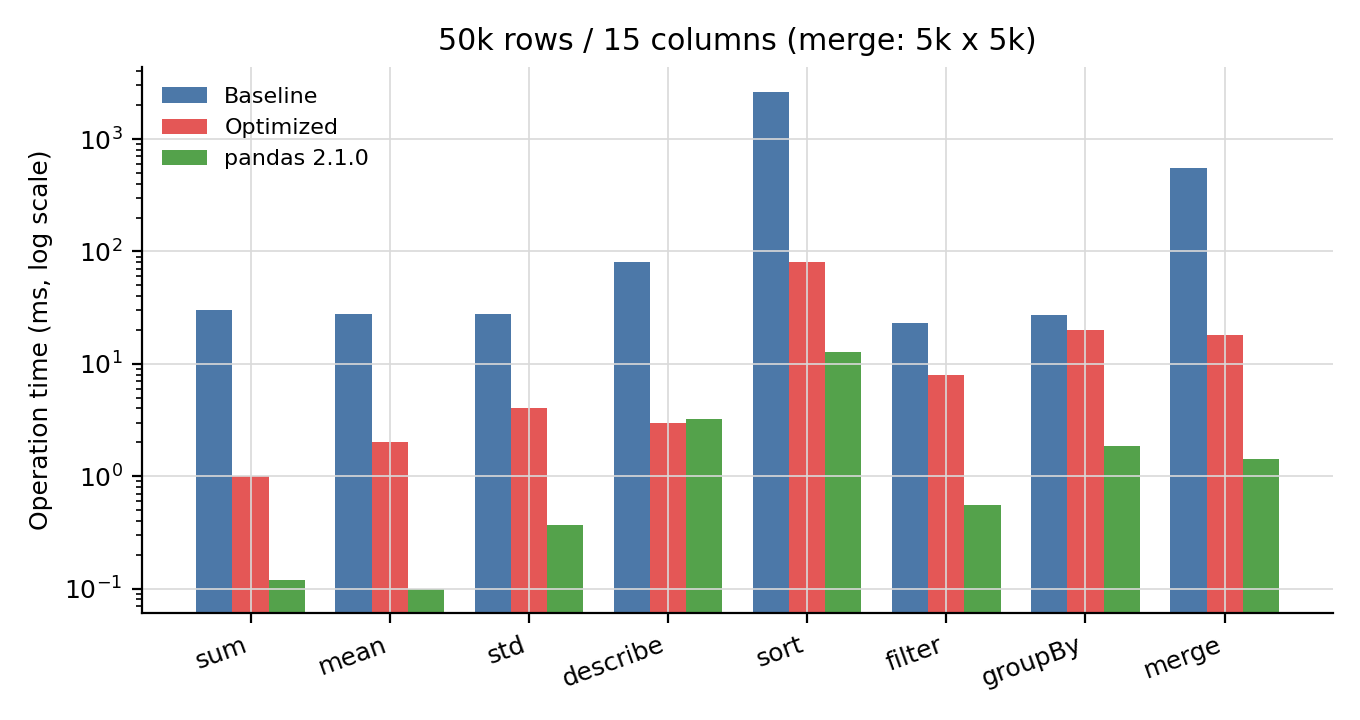
\includegraphics[width=0.88\linewidth]{figures/fig_ops_pandas.png}
\caption{Operation-time comparison with pandas 2.1.0 (log scale).}
\label{fig:pandasops}
\end{figure}

pandas remains 3.2--6.0$\times$ faster at reading.  Its memory increment, however, is higher than
the optimized retained heap: 106.8\,MB versus 56\,MB at 200k, 54.2\,MB versus 14\,MB at 50k.  The
comparison is not apples-to-apples: pandas runs in CPython with a C CSV parser and contiguous NumPy
arrays, while Andas runs on the JVM (and ART on Android), and RSS is not the same as a GC-retained
heap.  Still, it gives a useful upper bound.  The optimized implementation closes most of the
read-time gap of the baseline (roughly 10--14$\times$ slower than pandas) to 3.2--6.0$\times$, and
it uses less memory.  Computation kernels remain 6--20$\times$ slower than pandas, except
\code{describe}, which is slightly faster because pandas constructs several statistics and wraps
them in a Series.

\subsection{Cross-language consistency}

Performance is necessary but not sufficient: the same input must produce the same answer in
pandas, on the JVM, and on Android.  We extracted the first 5000 rows of the 50k dataset and
generated reference metrics with pandas 2.1.0.  The JVM harness and the Android instrumentation
test read the identical CSV (the Android copy is packaged as a test asset) and compute the same
35 metrics: cardinalities, `sum`/`mean`/`std`/`min`/`max`/`describe`, sort endpoints,
filter and group-by sums, join cardinality and amount, Pearson correlation, and normalized
endpoints.  Integer metrics must match exactly; floating-point metrics use a relative tolerance of
$10^{-10}$.

\begin{table}[t]
\centering
\footnotesize
\caption{Representative consistency metrics (pandas 2.1.0 vs JVM/Android).}
\label{tab:consistency}
\begin{tabular}{@{}lrrr@{}}
\toprule
Metric & pandas & JVM & Android \\
\midrule
\code{sum(d10)} & -7465.802624422415 & -7465.802624422438 & -7465.802624422438 \\
\code{std(d10)} & 57.606263335764076 & 57.60626333576399 & 57.60626333576399 \\
sort first value & -99.94711091909323 & -99.94711091909323 & -99.94711091909323 \\
filter count & 222 & 222 & 222 \\
\code{groupby cat\_3} & -2092.5884491227703 & -2092.588449122769 & -2092.588449122769 \\
merge rows & 5000 & 5000 & 5000 \\
\code{corr(d10,d11)} & 0.008147698079084498 & 0.008147698079084522 & 0.008147698079084522 \\
\bottomrule
\end{tabular}
\end{table}

All 35 metrics pass on both the JVM and Android.  The maximum relative error is
$3.17\times10^{-15}$, well below the $10^{-10}$ threshold; integer counts and sort endpoints match
exactly.  The residual difference is explained by floating-point summation order (NumPy pairwise
summation versus sequential accumulation), not by a semantic difference.  The full table is
provided in \path{bench/results/consistency_summary.csv}.

\subsection{Android emulator}

Table~\ref{tab:android} and Figure~\ref{fig:android} report the Android experiment.  The CSV is
generated on the device before the timed read; only the read is measured.

\begin{table}[H]
\centering
\small
\caption{Android emulator CSV read (API 36 ARM64, 192\,MB heap).}
\label{tab:android}
\begin{tabular}{@{}rrrrr@{}}
\toprule
Rows & Baseline (ms) & Optimized (ms) & Baseline retained (MB) & Optimized retained (MB) \\
\midrule
10k  & 1787 & 1192 & 10 & 1 \\
25k  & 3298 & 2025 & 28 & 4 \\
50k  & 6431 & 3468 & 56 & 8 \\
100k & OOM (18.1\,s) & 7317 & -- & 18 \\
200k & OOM (64.5\,s) & 16042 & -- & 35 \\
\bottomrule
\end{tabular}
\end{table}

\begin{figure}[H]
\centering
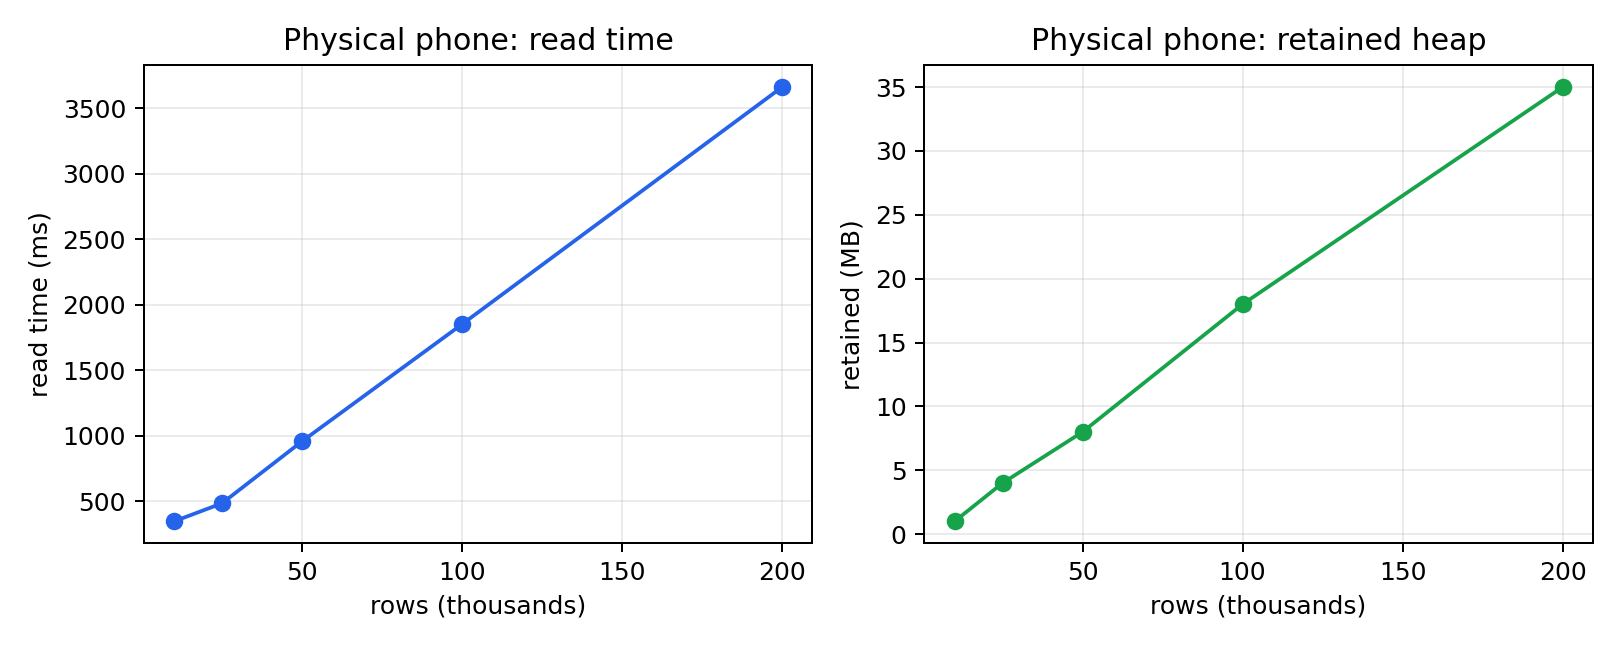
\includegraphics[width=0.95\linewidth]{figures/fig_report_android.png}
\caption{Android emulator results: (a) read time; (b) retained heap after GC.  The baseline OOMs
at 100k and 200k rows; the optimized reader completes 200k rows with 35\,MB of retained heap.}
\label{fig:android}
\end{figure}

The Android results reproduce the JVM trend and directly address the original failure.  The legacy
reader exhausts the 192\,MB heap at 100k rows after 18.1\,s and at 200k rows after 64.5\,s.  The
optimized reader completes 100k rows in 7.3\,s with 18\,MB retained and 200k rows in 16.0\,s with
35\,MB retained.  For the sizes that both complete, the read time falls by 33\%, 39\%, and 46\% at
10k, 25k, and 50k rows; retained memory falls by roughly 7$\times$ at 50k.

\subsection{Numeric engine: NumPy-style arrays and SciPy-style kernels}

The 0.2.0 preview adds a typed N-D array, linear algebra, FFT, statistics, regression, sparse
matrices, image filters, and a Matplotlib-style renderer.  We benchmarked the Kotlin fallback on
the JVM and the JNI path on the Android emulator against NumPy 1.26 on the same host (Apple M2,
Python 3.10.11).  Each operation is warmed up once and the median of three runs is reported; the
JVM uses a 2\,GB heap, Android uses the library's 192\,MB heap.

\begin{table}[t]
\centering
\footnotesize
\caption{Numeric kernel latency (ms, median).  JVM runs the Kotlin fallback; Android uses JNI
where available.  The last column is Android JNI versus the JVM fallback.}
\label{tab:numeric}
\begin{tabular}{@{}lrrrr@{}}
\toprule
Operation & NumPy & JVM fallback & Android JNI & JNI speedup \\
\midrule
add, 1M & 0.95 & 8.65 & 5.08 & 1.7$\times$ \\
sum, 1M & 0.22 & 2.03 & 1.38 & 1.5$\times$ \\
matmul, $300^2$ & 34.49 & 32.80 & 39.85 & 0.8$\times$ \\
FFT, 1024 & 0.008 & 17.36 & 0.28 & 62$\times$ \\
quantile, 1M & 32.90 & 92.30 & 109.40 & 0.8$\times$ \\
OLS, $20k\times5$ & 1.00 & 46.92 & 13.66 & 3.4$\times$ \\
convolve, $100k\times16$ & 0.75 & 4.52 & 1.47 & 3.1$\times$ \\
\bottomrule
\end{tabular}
\end{table}

The JNI path removes the quadratic DFT fallback: FFT drops from 17.4\,ms to 0.28\,ms, a
62$\times$ improvement, and the OLS normal-equation path benefits from native matmul
(46.9\,ms to 13.7\,ms).  Dense matmul is already competitive with NumPy; the remaining gaps are
dominated by JVM/Kotlin loop overhead and by the emulator's CPU, not by asymptotic complexity.
Quantile is intentionally a full sort in both implementations; the Android result includes
allocation and GC in the 192\,MB heap.

\subsection{Numeric cross-language consistency}

The numeric stack is checked against 43 reference values generated independently with NumPy,
\texttt{math.erf}, and an mpmath regularized incomplete beta for the t-test.  Inputs are
deterministic (an arithmetic sequence, fixed integer matrices, an 8-point FFT, and a 10-point
linear relation).  JVM and Android instrumentation tests read the same CSV reference table and
compare sums, moments, quantiles, determinant, linear solve, matmul, FFT coefficients,
convolution, OLS slope/intercept, normal CDF, and the t statistic/p-value.  Floating-point
metrics use a relative tolerance of $10^{-10}$ ($10^{-9}$ for FFT and the extreme t p-value);
all 43 pass on both runtimes.  This complements the pandas consistency experiment and covers
the new numeric code path rather than the CSV reader.

\section{Discussion}

\subsection{Memory complexity}

For $n$ rows, $m$ columns, and average string length $L$, the legacy design retains
$O(nm)$ map entries and boxed values, a transposed copy of the data, and $O(nm)$ index entries and
hash-map entries.  The optimized design retains $O(n)$ primitive values per numeric column,
$O(nL)$ characters for string columns, and one $O(1)$ or $O(n)$ index shared by all columns
($O(1)$ for the default range index).  This explains both the lower retained heap and the higher
row count that fits in a fixed heap.

\subsection{Where the speedups come from}

The gains are not uniformly due to JNI.  They come from:
\begin{itemize}
  \item removing intermediate lists and boxing in statistical kernels (7--30$\times$);
  \item changing sorting from quadratic label lookups to an $O(n\log n)$ permutation (32.9$\times$,
        with the gap growing with $n$);
  \item changing joins from nested loops to a hash join (30.9$\times$);
  \item streaming ingestion that avoids a full transposition (2--2.6$\times$).
\end{itemize}
Grouped sum improves only 1.4$\times$ because the legacy fallback already used a hash map.  This
heterogeneity is useful: it shows which operations were actually pathological and which were
already near their algorithmic optimum.

\subsection{Remaining gap and future work}

The comparison with pandas suggests three directions.  First, a native CSV tokenizer that parses
numbers directly from bytes and writes into off-heap arrays could reduce the remaining 3--6$\times$
read gap.  Second, vectorized native kernels over primitive columns could remove JNI call and
boxing overhead for statistics, filtering, and grouping.  Third, a zero-copy column format (for
example, an Arrow-compatible buffer) would allow interop with other tools and avoid materializing
the \code{List} view.  On Android, ART's JIT and GC behavior also deserve a dedicated study on
physical devices, since our measurements use an emulator.

\section{Threats to Validity}

\begin{enumerate}
  \item \textbf{JVM versus ART.}  JVM measurements do not fully represent ART's JIT and GC behavior.
        We mitigate this with an Android emulator experiment, but an emulator is still not a phone.
  \item \textbf{Baseline JVM fallback.}  The JVM has no native library, so the baseline is patched
        to fall back to Kotlin.  This affects absolute times for kernels that would otherwise use
        JNI.  The Android read experiment uses the unmodified baseline, so the read conclusions are
        unaffected.
  \item \textbf{Synthetic data.}  The data distribution and string lengths differ from production
        workloads.  The generator is seeded and deterministic, and the schema mirrors the project's
        real 37\,MB file; we also exercise that file in unit tests.
  \item \textbf{Peak sampling.}  A 50\,ms sampler can miss short peaks, and \code{System.gc()} does
        not guarantee immediate collection.  Retained values can fluctuate by a few megabytes.
  \item \textbf{pandas runtime differences.}  pandas runs on CPython with C/NumPy, while Andas runs
        on the JVM/ART.  Memory is reported as RSS increment for pandas and retained heap for Andas.
        The comparison is intended as an order-of-magnitude reference, not a claim that one library
        is universally faster.
  \item \textbf{Single-machine study.}  Each configuration is repeated three times and we report
        medians, but we do not repeat the study across machines or device models.
\end{enumerate}

\section{Related Work}

pandas established the \code{DataFrame} abstraction for Python and remains the reference API for
tabular data analysis \cite{pandas}.  Columnar in-memory formats such as Apache Arrow \cite{arrow}
motivate contiguous primitive buffers and zero-copy interchange; Andas adopts the columnar idea but
keeps a Kotlin/JVM API.  On Android, most data-processing libraries either wrap SQLite or operate on
row-oriented collections; Andas targets analytic operations over in-memory columns.  The JVM
ecosystem offers high-performance collections and off-heap buffers, which are natural next steps for
the native kernels described in Section~6.3.

\section{Conclusion}

The legacy Andas reader was limited by memory amplification, not by CPU speed.  Materializing the
whole file, building row maps, transposing into columns, and duplicating indices made a 36\,MB file
unreadable on a 192\,MB Android heap.  Streaming columnar ingestion, a shared index, primitive
storage, and algorithmic rewrites raise the readable size to 200k rows with 35\,MB of retained heap
on Android, and to 200k rows with 56\,MB on a 256\,MB JVM heap.  At 50k rows, statistical and
sorting kernels improve by 7--33$\times$ and hash joins by 30.9$\times$.  pandas remains faster on
the desktop because of its C/NumPy engine, but the optimized library narrows the read gap and uses
less memory.  A 35-metric cross-language consistency check against pandas passes on both the JVM
and Android with a maximum relative error of $3.17\times10^{-15}$.  The remaining 6--20$\times$
kernel gap motivates native columnar kernels and zero-copy buffers as future work.

\appendix
\section{Reproducibility}

The repository contains the benchmark scripts, raw results, and figures.  The main commands are:

\begin{lstlisting}[language=bash]
python3 bench/gen_data.py
./bench/prepare_baseline.sh 9bb6715
python3 bench/run_benchmarks.py
python3 bench/run_pandas_benchmarks.py
python3 bench/compare_pandas.py
python3 bench/plot_results.py
\end{lstlisting}

The Android experiment is an instrumentation test:

\begin{lstlisting}[language=bash]
export ANDROID_USER_HOME="$PWD/.android-home"
TEST=cn.ac.oac.libs.andas.CsvBenchInstrumentedTest
adb logcat -c
./gradlew :android-pandas:connectedDebugAndroidTest \
  -Pandroid.testInstrumentationRunnerArguments.class=$TEST
adb logcat -d -s ANDAS_BENCH:I
\end{lstlisting}

Raw JVM results, pandas comparison tables, and Android logcat output are stored under
\path{bench/results/}.  The LaTeX source of this report is in \path{report/} and can be rebuilt
with \code{latexmk -pdf andas-technical-report.tex}.

\begin{thebibliography}{9}
\bibitem{pandas}
W.~McKinney, ``Data Structures for Statistical Computing in Python,''
in \emph{Proceedings of the 9th Python in Science Conference}, 2010, pp.~56--61.

\bibitem{pandasdocs}
pandas Development Team, ``pandas: powerful Python data analysis toolkit,''
\url{https://pandas.pydata.org/}, 2026.

\bibitem{kotlin}
JetBrains, ``Kotlin Programming Language,'' \url{https://kotlinlang.org/}, 2026.

\bibitem{android}
Google, ``Android Runtime (ART) and Dalvik,'' \url{https://source.android.com/docs/core/runtime}, 2026.

\bibitem{arrow}
Apache Software Foundation, ``Apache Arrow: A cross-language development platform for in-memory
data,'' \url{https://arrow.apache.org/}, 2026.

\bibitem{jmh}
Oracle, ``Java Microbenchmark Harness (JMH),'' \url{https://openjdk.org/projects/code-tools/jmh/}, 2026.
\end{thebibliography}

\end{document}
